
Šiame magistro baigiamame darbe yra palyginami 4 neuroninių tinklų architektūros: daugiavaizdis neuroninis tinklas, aprašytas poskyryje "Daugiavaizdis konvoliucinis neuroninis tinklas", kapsulinis neuroninis tinklas, aprašytas poskyryje "Tiriamo kapsulinio neuroninio tinklo architektūra", ir 2 daugiavaizdžiai kapsuliniai neuroniniai tinklai, aprašyti poskyriuose "Tiriamo daugiavaizdžio kapsulinio neuroninio tinklo architektūra su vaizdų sujungimo sluoksniu" ir "Tiriamo daugiavaizdžio kapsulinio neuroninio tinklo architektūra su vaizdų kapsuliniu sluoksniu". Kiekvienas tiriamas dirbtinis neuroninis tinklas yra apmokomas naudojantis visais duomenimis, aprašytais poskyryje Tyrimams naudoti duomenys. Šie duomenys apmokymo metu yra padalinami į duomenų rinkinius, iš kurių kiekvienas yra sudarytas iš 96 2D nuotraukų. Daugiavaizdžio konvoliucinio ir kapsulinio neuroninių tinklų apmokymų antram etapui duomenų rinkiniai sudaryti iš nuotraukų grupių, kuriose yra visos konkretaus 3D objekto modelio nuotraukos. Kiekvienas dirbtinis neuroninis tinklas yra apmokomas per 10 epochų. Daugiavaizdžio konvoliucinio ir kapsulinio neuroninių tinklų abu apmokymo etapai yra apmokomi po 5 epochas.

Visų šiame magistro baigiamame darbe tiriamų dirbtinių neuroninių tinklų apmokymai trunka po 6-7 valandas naudojantis Kaggle sistema. Šioje sistemoje vartotojui yra išskiriama viena Nvidia Tesla P100 vaizdo plokštė, kuri turi 3584 CUDA branduolių ir 16 GB RAM atminties. Taip pat šioje sistemoje vartotojui yra suteikiamas Intel(R) Xeon(R) CPU, kuris turi vieną branduolį, 39,424 MB spartinančiosios atminties ir kurio dažnis yra 2000,176 MHz. Galiausiai ši sistema vartotojui išskiria 16,4 GB RAM atminties.

Šiame magistro baigiamame darbe bandoma optimizuoti kapsulinių neuroninių tinklų modifikacijų konfigūracijas. Pirmiausia bandoma optimizuoti šiuos tinklus naudojantis Bajeso hiperparametrų optimizavimo algoritmu, kuris yra aprašytas darbe \cite{bayes}. Toliau bandomos kitos konfigūracijos nei konfigūracijos aprašytos darbe \cite{capsNet}. Tačiau, dėl Kaggle sistemos apribojimų, nei vienas metodas neaptiko geresnių kapsulinių neuroninių tinklų modifikacijų konfigūracijų. Taip pat bandoma 
keisti mokymosi greitį. Tačiau skirtumai tarp rezultatų yra nereikšmingi.

Po kiekvienos epochos yra renkamos tikslumo metrikos: tikslumas klasifikuojant apmokymo duomenis, ši informacija pavaizduota \ref{tbl:train} lentelėje ir \ref{img:train_plot} paveikslėlyje, ir tikslumas klasifikuojant testavimo duomenis, ši informacija atvaizduota \ref{tbl:valid} lentelėje ir \ref{img:val_plot} paveikslėlyje. Tikslumas yra teisingai suklasifikuotų įrašų dalis klasifikuotų duomenų aibėje. \ref{tbl:train}, \ref{tbl:valid} lentelių stulpelio pavaidinimas ir \ref{img:train_plot}, \ref{img:val_plot} grafikų kreivių pavadinimas mvcnn yra daugiavaizdžio neuroninio tinklo tikslumas, capsnet - kapsulinio neuroninio tinklo tikslumas, mv\_capsnet - daugiavaizdžio kapsulinio neuroninio tinklo su vaizdų sujungimo sluoksniu tikslumas, mv\_cap\_capsnet1 - daugiavaizdžio kapsulinio neuroninio tinklo su vaizdų kapsuliniu sluoksniu ir vienu mokymosi etapu tikslumas, mv\_cap\_capsnet2 - daugiavaizdžio kapsulinio neuroninio tinklo su vaizdų kapsuliniu sluoksniu ir dviem mokymosi etapais tikslumas. Brūkšninė vertikali linija \ref{img:train_plot} ir \ref{img:val_plot} grafikuose nurodo antrojo apmokymo etapo pirmąją epochą.

\begin{table}[]
\begin{tabular}{l|l|l|l|l|l}
	epocha &     mvcnn &   capsnet & mv\_capsnet & mv\_cap\_capsnet1 & mv\_cap\_capsnet2 \\ \hline
	1 & 0,688 &   0,119 &      0,517 &           0,281 &           0,218 \\
	2 & 0,860 &   0,529 &      0,793 &           0,807 &           0,624 \\
	3 & 0,904 &   0,660 &      0,840 &           0,880 &           0,731 \\
	4 & 0,929 &   0,720 &      0,871 &           0,911 &           0,785 \\
	5 & 0,944 &   0,758 &      0,895 &           0,933 &           0,821 \\
	6 & 0,937 &   0,783 &      0,878 &           0,948 &           0,717 \\
	7 & 0,950 &   0,805 &      0,929 &           0,958 &           0,911 \\
	8 & 0,959 &   0,821 &      0,952 &           0,965 &           0,944 \\
	9 & 0,961 &   0,835 &      0,966 &           0,970 &           0,962 \\
	10 & \textbf{0,972} &   \textbf{0,847} &      \textbf{0,972} &           \textbf{0,975} &           \textbf{0,970} \\
\end{tabular}
\caption{
	Apmokymo duomenų klasifikavimo tikslumas, kur mvcnn yra daugiavaizdžio neuroninio tinklo tikslumas, capsnet - kapsulinio neuroninio tinklo tikslumas, mv\_capsnet - daugiavaizdžio kapsulinio neuroninio tinklo su vaizdų sujungimo sluoksniu tikslumas, mv\_cap\_capsnet1 - daugiavaizdžio kapsulinio neuroninio tinklo su vaizdų kapsuliniu sluoksniu ir vienu mokymosi etapu tikslumas, mv\_cap\_capsnet2 - daugiavaizdžio kapsulinio neuroninio tinklo su vaizdų kapsuliniu sluoksniu ir dviem mokymosi etapais tikslumas. Kiekviename stulpelyje geriausi pasiekti tikslumai yra paryškinti.
}
\label{tbl:train}
\end{table}

\begin{table}[]
\begin{tabular}{l|l|l|l|l|l}
	epocha &     mvcnn &   capsnet & mv\_capsnet & mv\_cap\_capsnet1 & mv\_cap\_capsnet2 \\ \hline
	1 & 0,792 &   0,302 &      0,718 &           0,692 &           0,480 \\
	2 & 0,835 &   0,562 &      0,768 &           0,789 &           0,629 \\
	3 & 0,849 &   0,631 &      0,778 &           0,822 &           0,687 \\
	4 & 0,858 &   0,663 &      0,784 &           0,828 &           0,714 \\
	5 & 0,860 &   0,683 &      0,800 &           0,850 &           0,721 \\
	6 & 0,888 &   0,674 &      0,800 &           0,861 &           0,832 \\
	7 & 0,880 &   0,698 &      0,822 &           \textbf{0,864} &          \textbf{0,848} \\
	8 & 0,881 &   0,701 &      0,827 &           0,862 &           0,838 \\
	9 & 0,896 &   \textbf{0,723} &      0,808 &           0,861 &           0,841 \\
	10 & \textbf{0,901} &   0,710 &      \textbf{0,853} &           0,856 &           0,828 \\
\end{tabular}
\caption{
	Testavimo duomenų klasifikavimo tikslumas, kur mvcnn yra daugiavaizdžio neuroninio tinklo tikslumas, capsnet - kapsulinio neuroninio tinklo tikslumas, mv\_capsnet - daugiavaizdžio kapsulinio neuroninio tinklo su vaizdų sujungimo sluoksniu tikslumas, mv\_cap\_capsnet1 - daugiavaizdžio kapsulinio neuroninio tinklo su vaizdų kapsuliniu sluoksniu ir vienu mokymosi etapu tikslumas, mv\_cap\_capsnet2 - daugiavaizdžio kapsulinio neuroninio tinklo su vaizdų kapsuliniu sluoksniu ir dviem mokymosi etapais tikslumas. Kiekviename stulpelyje geriausi pasiekti tikslumai yra paryškinti.
}
\label{tbl:valid}
\end{table}

\begin{figure}[H]
	\centering
	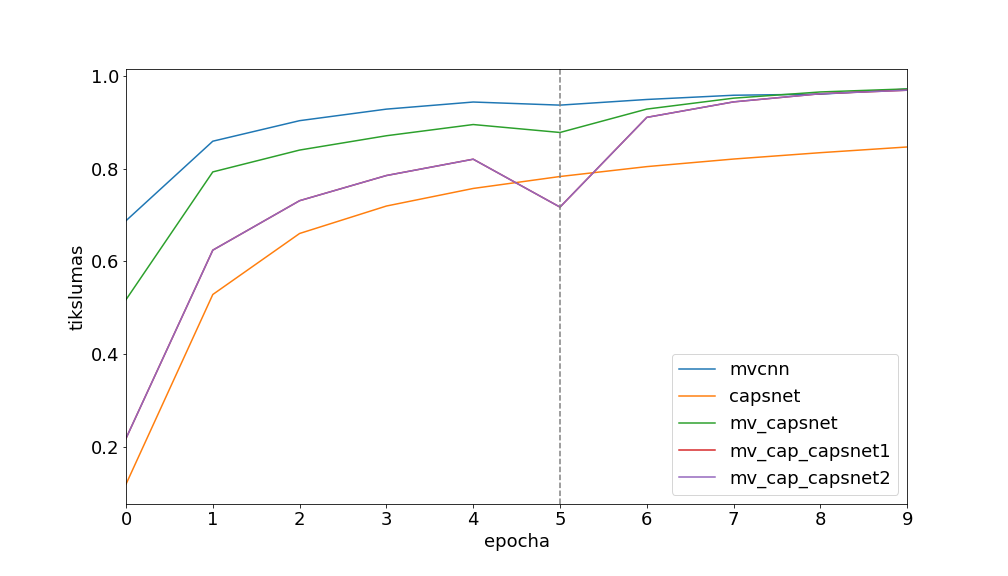
\includegraphics[scale=0.5]{img/trained.png}
	\caption{
		Apmokymo duomenų klasifikavimo tikslumas, kur mvcnn yra daugiavaizdžio neuroninio tinklo tikslumas, capsnet - kapsulinio neuroninio tinklo tikslumas, mv\_capsnet - daugiavaizdžio kapsulinio neuroninio tinklo su vaizdų sujungimo sluoksniu tikslumas, mv\_cap\_capsnet1 - daugiavaizdžio kapsulinio neuroninio tinklo su vaizdų kapsuliniu sluoksniu ir vienu mokymosi etapu tikslumas, mv\_cap\_capsnet2 - daugiavaizdžio kapsulinio neuroninio tinklo su vaizdų kapsuliniu sluoksniu ir dviem mokymosi etapais tikslumas. Brūkšninė vertikali linija nurodo antrojo apmokymo etapo pirmąją epochą.
	}
	\label{img:train_plot}
\end{figure}

\begin{figure}[H]
	\centering
	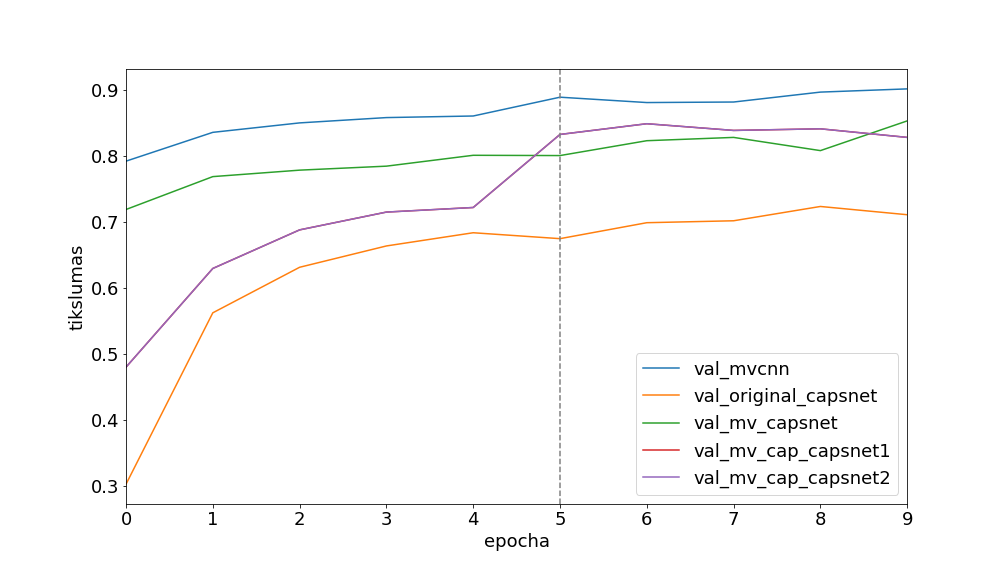
\includegraphics[scale=0.5]{img/validated.png}
	\caption{
		Testavimo duomenų klasifikavimo tikslumas, kur mvcnn yra daugiavaizdžio neuroninio tinklo tikslumas, capsnet - kapsulinio neuroninio tinklo tikslumas, mv\_capsnet - daugiavaizdžio kapsulinio neuroninio tinklo su vaizdų sujungimo sluoksniu tikslumas, mv\_cap\_capsnet1 - daugiavaizdžio kapsulinio neuroninio tinklo su vaizdų kapsuliniu sluoksniu ir vienu mokymosi etapu tikslumas, mv\_cap\_capsnet2 - daugiavaizdžio kapsulinio neuroninio tinklo su vaizdų kapsuliniu sluoksniu ir dviem mokymosi etapais tikslumas. Brūkšninė vertikali linija nurodo antrojo apmokymo etapo pirmąją epochą.
	}
	\label{img:val_plot}
\end{figure}

Darbe \cite{capsNet} yra teigiama, kad kapsuliniai neuroniniai tinklai reikalauja mažesnės apmokymo duomenų imties nei konvoliuciniai neuroniniai tinklai. Todėl šiame magistro baigiamame darbe yra atliekami tyrimai su tyrimų duomenų poaibiais. Tiriami tik daugiavaizdis neuroninis tinklas ir daugiavaizdis kapsulinis neuroninis tinklas su vaizdų kapsuliniu sluoksniu ir vienu mokymosi etapu. Lentelėje \ref{tbl:less_datav1} ir grafike \ref{img:less_datav1} pavaizduoti tyrimų rezultatai su apmokymo duomenimis, sudarytais iš 4904 3D objektų modelių, ir testavimo 1232. Lentelėje \ref{tbl:less_datav2} ir grafike \ref{img:less_datav2} pavaizduoti tyrimų rezultatai su apmokymo duomenimis, sudarytais iš 3264 3D objektų modelių, ir testavimo 2464. Šių lentelių stulpelio pavadinimas ir grafikų kreivės pavadinimas mvcnn yra daugiavaizdžio neuroninio tinklo tikslumas klasifikuojant apmokymo duomenis, val\_mvcnn - daugiavaizdžio neuroninio tinklo tikslumas klasifikuojant testavimo duomenis, mv\_cap\_capsnet - daugiavaizdžio kapsulinio neuroninio tinklo su vaizdų kapsuliniu sluoksniu ir vienu mokymosi etapu tikslumas klasifikuojant apmokymo duomenis, val\_mv\_cap\_capsnet - daugiavaizdžio kapsulinio neuroninio tinklo su vaizdų kapsuliniu sluoksniu ir vienu mokymosi etapu tikslumas klasifikuojant testavimo duomenis. Brūkšninė vertikali linija grafikuose nurodo antrojo apmokymo etapo pirmąją epochą.

\begin{table}[]
	\begin{tabular}{l|l|l|l|l}
		epocha &     mvcnn & val\_mvcnn & mv\_cap\_capsnet & val\_mv\_cap\_capsnet \\ \hline
		 1 & 0,594 &     0,752 &          0,064 &              0,041 \\
		2 & 0,821 &     0,792 &          0,219 &              0,532 \\
		3 & 0,875 &     0,816 &          0,706 &              0,742 \\
		4 & 0,910 &     0,824 &          0,813 &              0,801 \\
		5 & 0,930 &     0,819 &          0,878 &              0,810 \\
		6 & 0,922 &     0,836 &          0,910 &              0,826 \\
		7 & 0,928 &     0,847 &          0,930 &              0,828 \\
		8 & 0,948 &     0,862 &          0,944 &              0,831 \\
		9 & 0,955 &     \textbf{0,868} &          0,956 &              0,829 \\
		10 & \textbf{0,961} &     0,847 &          \textbf{0,964} &              \textbf{0,832} \\
	\end{tabular}
	\caption{
		Tyrimų rezultatai su apmokymo duomenimis, sudarytais iš 4904 3D objektų modelių, ir testavimo 1232, kur mvcnn yra daugiavaizdžio neuroninio tinklo tikslumas klasifikuojant apmokymo duomenis, val\_mvcnn - daugiavaizdžio neuroninio tinklo tikslumas klasifikuojant testavimo duomenis, mv\_cap\_capsnet - daugiavaizdžio kapsulinio neuroninio tinklo su vaizdų kapsuliniu sluoksniu ir vienu mokymosi etapu tikslumas klasifikuojant apmokymo duomenis, val\_mv\_cap\_capsnet - daugiavaizdžio kapsulinio neuroninio tinklo su vaizdų kapsuliniu sluoksniu ir vienu mokymosi etapu tikslumas klasifikuojant testavimo duomenis. Kiekviename stulpelyje geriausi pasiekti tikslumai yra paryškinti.
	}
	\label{tbl:less_datav1}
\end{table}


\begin{figure}[H]
	\centering
	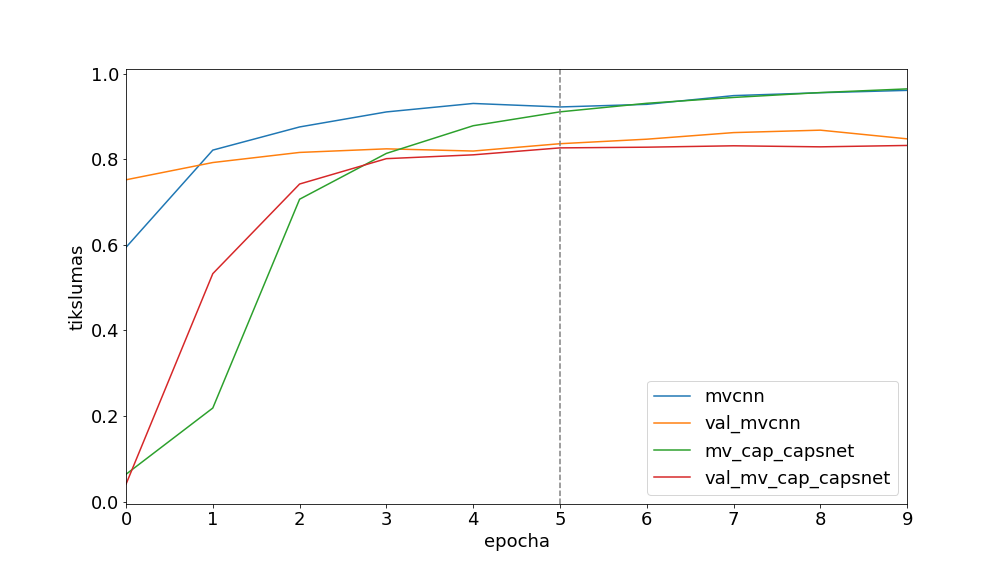
\includegraphics[scale=0.5]{img/less_data_v1.png}
	\caption{
		Tyrimų rezultatai su apmokymo duomenimis, sudarytais iš 4904 3D objektų modelių, ir testavimo 1232, kur mvcnn yra daugiavaizdžio neuroninio tinklo tikslumas klasifikuojant apmokymo duomenis, val\_mvcnn - daugiavaizdžio neuroninio tinklo tikslumas klasifikuojant testavimo duomenis, mv\_cap\_capsnet - daugiavaizdžio kapsulinio neuroninio tinklo su vaizdų kapsuliniu sluoksniu ir vienu mokymosi etapu tikslumas klasifikuojant apmokymo duomenis, val\_mv\_cap\_capsnet - daugiavaizdžio kapsulinio neuroninio tinklo su vaizdų kapsuliniu sluoksniu ir vienu mokymosi etapu tikslumas klasifikuojant testavimo duomenis. Brūkšninė vertikali linija grafikuose nurodo antrojo apmokymo etapo pirmąją epochą.
	}
	\label{img:less_datav1}
\end{figure}

\begin{table}[]
	\begin{tabular}{l|l|l|l|l}
		epocha &     mvcnn & val\_mvcnn & mv\_cap\_capsnet & val\_mv\_cap\_capsnet \\ \hline
		1 & 0,511 &     0,706 &          0,065 &              0,041 \\
		2 & 0,775 &     0,767 &          0,380 &              0,571 \\
		3 & 0,850 &     0,798 &          0,727 &              0,696 \\
		4 & 0,889 &     0,805 &          0,817 &              0,739 \\
		5 & 0,916 &     0,813 &          0,874 &              0,762 \\
		6 & 0,910 &     0,832 &          0,907 &              0,772 \\
		7 & 0,915 &     0,808 &          0,929 &              0,781 \\
		8 & 0,936 &     0,822 &          0,946 &              0,807 \\
		9 & 0,943 &     0,851 &          0,957 &              0,808 \\
		10 & \textbf{0,951} &     \textbf{0,853} &         \textbf{0,965} &              \textbf{0,816} \\
	\end{tabular}
	\caption{
		Tyrimų rezultatai su apmokymo duomenimis, sudarytais iš 3264 3D objektų modelių, ir testavimo 2464, kur mvcnn yra daugiavaizdžio neuroninio tinklo tikslumas klasifikuojant apmokymo duomenis, val\_mvcnn - daugiavaizdžio neuroninio tinklo tikslumas klasifikuojant testavimo duomenis, mv\_cap\_capsnet - daugiavaizdžio kapsulinio neuroninio tinklo su vaizdų kapsuliniu sluoksniu ir vienu mokymosi etapu tikslumas klasifikuojant apmokymo duomenis, val\_mv\_cap\_capsnet - daugiavaizdžio kapsulinio neuroninio tinklo su vaizdų kapsuliniu sluoksniu ir vienu mokymosi etapu tikslumas klasifikuojant testavimo duomenis. Kiekviename stulpelyje geriausi pasiekti tikslumai yra paryškinti.
	}
	\label{tbl:less_datav2}
\end{table}


\begin{figure}[H]
	\centering
	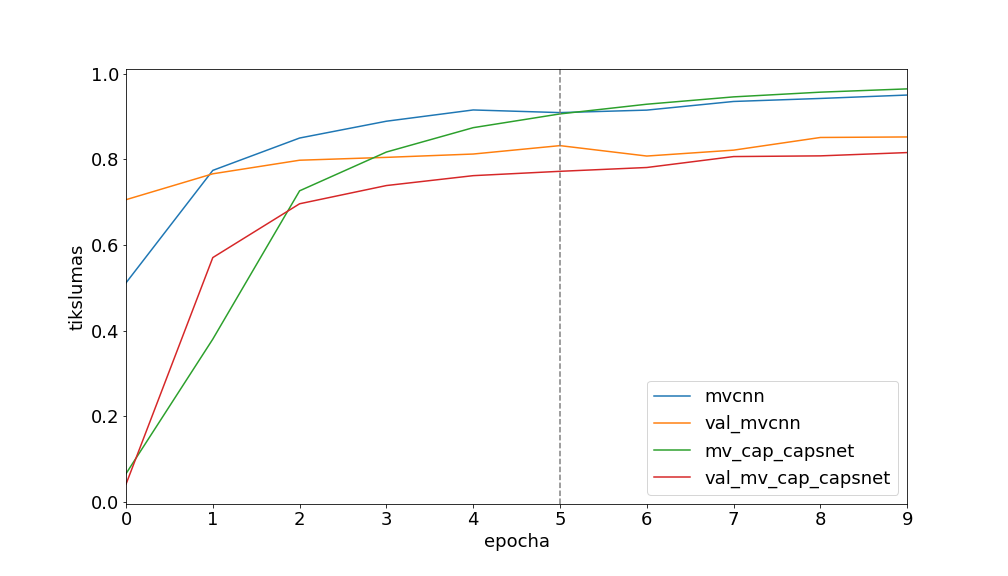
\includegraphics[scale=0.5]{img/less_data_v2.png}
	\caption{
		Tyrimų rezultatai su apmokymo duomenimis, sudarytais iš 3264 3D objektų modelių, ir testavimo 2464, kur mvcnn yra daugiavaizdžio neuroninio tinklo tikslumas klasifikuojant apmokymo duomenis, val\_mvcnn - daugiavaizdžio neuroninio tinklo tikslumas klasifikuojant testavimo duomenis, mv\_cap\_capsnet - daugiavaizdžio kapsulinio neuroninio tinklo su vaizdų kapsuliniu sluoksniu ir vienu mokymosi etapu tikslumas klasifikuojant apmokymo duomenis, val\_mv\_cap\_capsnet - daugiavaizdžio kapsulinio neuroninio tinklo su vaizdų kapsuliniu sluoksniu ir vienu mokymosi etapu tikslumas klasifikuojant testavimo duomenis.	Brūkšninė vertikali linija grafikuose nurodo antrojo apmokymo etapo pirmąją epochą.
	}
	\label{img:less_datav2}
\end{figure}


